\documentclass[a4paper,10pt]{article}
%\usepackage{fancyvrb,relsize}
\usepackage[small,compact]{titlesec}
\usepackage[pdftex]{graphicx}
\usepackage{listings}
\usepackage{natbib}
\lstset{language=C}
%\usepackage[margin=3.50cm]{geometry}
\linespread{1.1}
\setlength{\parindent}{0pt}
\setlength{\parskip}{0.5ex plus 0.5ex minus 0.3ex}
\sloppy
\setlength{\oddsidemargin}{0in} \setlength{\evensidemargin}{0in}
\setlength{\textwidth}{6.5in} \setlength{\textheight}{9.5in}
\setlength{\topmargin}{-0.65in}
\setlength\bibsep{0.1cm}

\begin{document}

\begin{center}
{\bf A Framework For Realizing Autoparallelism\\ Through Automatic OpenMP Code Generation}\\
\end{center}
%\vspace{0.1cm}
  \begin{tabbing}
      1111111111111111111111111111 \= 111111111111111 \= 1111\kill
   {\bf Name} \> : Raghesh A\\
   {\bf Reg. No} \> : CS09M032\\
   {\bf Registered for} \> : MTech\\
   {\bf Project Guide} \> : Dr.Shankar Balachandran \\
   {\bf Project Area} \> :  Compiler Optimization\\
   {\bf Date} \> :  21-01-2011\\
  \end{tabbing} 
\begin{abstract}
A framework for automatically generating OpenMP code after detecting parallelism
in programs is proposed. The approach is independent of the programming language.
A performance similar to that of a program which has OpenMP
pragmas provided by the user is observed. It is expected to get more performance
with the integration of profile guided optimization into this.
\end{abstract}
\section{Introduction}
The framework is implemented using Polly\cite{pollywiki}, an open source\cite{lice}
compiler optimization framework that uses a
mathematical representation, the polyhedral model, to represent and transform
loops and other control flow
structures. It is an effort towards achieving autoparallelism in programs. The
transformations are being implemented in LLVM(Low level virtual machine)\cite{llvm}.
LLVM defines a common, low-level code representation in Static Single Assignment
(SSA) form, with several novel features. The LLVM compiler framework and
code representation together provide a combination of key capabilities that are
important for practical, lifelong analysis and transformation of programs. One
of the important features of LLVM is that the output of all the transformation
passes have same intermediate representation(LLVM IR), which makes the programmer's life
simple.
\begin{figure}[h]
\begin{center}
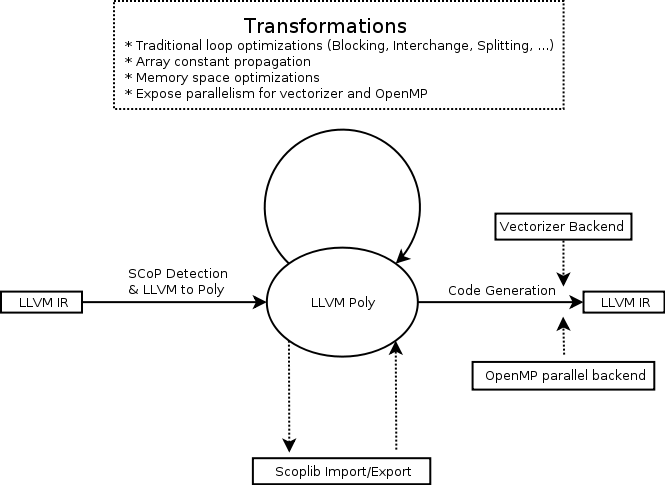
\includegraphics[scale=0.40]{LLVMPoly.png}
\caption{Polly Architecture}
\end{center}
\end{figure}

This document describes the work done for integrating a module for OpenMP\cite{openmp} code
generation in Polly. Input to Polly is the representation of the source program in LLVM IR. Polly
analyses it and finds regions, which can be parallelised. Necessary polyhedral transformations are made on this.
The region is called SCoP(Static Control Part)\cite{scop}, the
largest part of the code that can be represented in the polyhedral model\cite{pluto}.
The region doesn't contain irregular memory accesses, irregular 
control flow, statements with side effects, non pure function calls, etc. 
The OpenMP code generation module emits library calls(libgomp)\cite{libgomp} corresponding to these parallel regions.
The architecture is shown in Figure 1.

We are getting the performance similar to that of a program which has OpenMP
pragmas provided by the user. The advantage of Polly is that the parallelism 
is detected automatically without any user intervention. Also it is independent
of the programming language used because it works on LLVM IR.

\section{Work Done: OpenMP Code Generation for Polly}
In this section the work done for generating OpenMP code through Polly is 
described.
\subsection{Understanding Polly Codebase}
In order to understand the existing code of Polly an exercise is done to analyze
LLVM IR generated and to eliminate dead code from it. But after looking into the
code it is realized that it was already done as part of dependency analysis in
Polly. But this effort was really useful to understand the way of coding in Polly.
\subsection{Implementation}
Optimizations in Polly should be able to create loops that are executed in
parallel, as if the user would have added some OpenMP pragmas. To achieve this,
code generation needs to emit code that calls an OpenMP library to be executed
in parallel. The GNU OpenMP Library(libgomp) is used for this purpose. 
The dependency analysis module of Polly automatically 
detects parallel loops(SCoPs) and are given to OpenMP code generation module. 
Here we generate the required libgomp library calls. The code generated is 
similar the code generated if the user have added OpenMP pragmas\cite{parfor}.
The following sections explain the steps taken towards generating the OpenMP
code.  The generated code is in LLVM IR format. 

\subsubsection{Generating OpenMP Library Calls}
Consider the for loop below to have a basic understanding about what is to be done.

%\begin{verbatim}
{\footnotesize
\begin{lstlisting}
  for (int i = 0; i <= N; i++)
      A[i] = 1;
\end{lstlisting}
}
%\end{verbatim}

The above for loop is detected as a parallel loop and given for OpenMP code
generation. Here the following sequence of GOMP library calls with proper arguments and return types(signature)
has to be generated in LLVM IR format\cite{kaleid}.

{\small
\begin{itemize}
\item GOMP\_parallel\_loop\_runtime\_start
\item subfunction
\item GOMP\_parallel\_end
\end{itemize}
}
The code for body of the for loop is generated inside the subfunction which has
the following GOMP library calls to achieve the necessary parallelism.
{\small
\begin{itemize}
\item GOMP\_loop\_runtime\_next
\item GOMP\_loop\_end\_nowait
\end{itemize}
}
The signature and descriptions of each of the above functions can be 
found in in libgomp manual\cite{libgomp}.

\subsubsection{Support for inner loops}
So far OpenMP code created apply only for outer loops, which is detected as SCoP.
Next step is to do it for inner loops. Due to dependency issues the
outer loop is not detected as SCoP, but innerloop can be safely parallelized as
in the following example.
%\begin{verbatim}
{\footnotesize
\begin{lstlisting}
  for (int i = 0; i < N; i++) {
    for (int j = 0; j < N; j++) {
      A[j] += i;
    }
  }
\end{lstlisting}
}
%\end{verbatim}
Those loops need the values of the surrounding induction variables in the 
OpenMP subfunction. We need to pass the values of the outer induction 
variables in a structure to the subfunction. This step is almost completed with some minor issues to be fixed.

\subsection{Patches Committed To Polly}
For each of steps explained above a patch is committed to Polly repository and is
peer reviewed by Polly developers.
\subsection{Running Polly With OpenMP Enabled}
If we want to run Polly on some programs(test.c) install the required libraries by
following the steps here [12] and then issue the commands below.

{\footnotesize
  \$ clang -emit-llvm -S test.c\\
  \$ opt -mem2reg -polly-codegen -enable-polly-openmp test.s -S {\tiny $>$} test.ll\\
  \$ llc test.ll -o test.s\\
  \$ llvm-gcc-4.2 test.s -lgomp\\
  \$ ./a.out
}
\section{Results Obtained}
The following loop is tested on different machines and the results are shown in the table.
%\begin{verbatim}
{\footnotesize
\begin{lstlisting}
  for (i = 0; i < 1024; i++) {
    for (j = 0; j < 5000000; j++)
      A[i] += j;
  }
\end{lstlisting}
}
%\end{verbatim}
The comparison is made in four different machines with the code compiled with
{\footnotesize
\begin{itemize}
\item Clang\cite{clang} which generates only serial code (Serial Execution).
\item Polly with OpenMP enabled which generates necessary OpenMP code automatically(Automatic Parallelization).
\item GCC with OpenMP enabled. Here the user have to give the OpenMP pragmas manually(Manual Parallelization).
\end{itemize}
}
\begin{table}[h]
\begin{center}
{\footnotesize
\begin{tabular}{| l | p{2cm} | p{2cm} | p{2cm} | p{2cm} |}
\hline
& \textbf{Serial Execution} & \textbf{Automatic Parallelization(Polly)} & \textbf{Manual Parallelization(GCC)} \\ \hline
\textbf{Intel Core 2 Duo}(32 Bit OS)& 9.509s & 4.852s & 4.835s \\ \hline
\textbf{Intel Core 2 Duo}(64 Bit OS)& 6.40s  & 3.32s & 3.50s\\ \hline
\textbf{Intel Core i5}(64 Bit OS)   & 6.96s  & 3.78s & 3.75s\\ \hline
\textbf{AMD Engineering Sample(24 Core)}(64 Bit OS)   & 17.039s & 0.757s & 0.796s\\
\hline
\end{tabular}
}
\end{center}
\caption{Performance Comparison}
\end{table}
It can be observed that when OpenMP is enabled in Polly we are getting a performance
almost similar to GCC  with OpenMP pragmas provided by the user manually, which is the expected result. More
speedup is obtained in the 24 Core machine.
\section{Work Plan}
All or some of the features described below will be added to Polly. Third and fourth
proposals are of less academic interest and so it will be given lower priority.
\subsection{Integrating Profile Guided Optimization into Polly}
An improvement that can be made to Polly is integrating profile guided optimization
\cite{pgo}. The idea is explained below with a few examples. Consider the following code.
%\begin{verbatim}
{\footnotesize
\begin{lstlisting}
  scanf("%d", &b);
  for(i = 0; i < N; i +=  b) {
      body;
  }
\end{lstlisting}
}
%\end{verbatim}
Polly will not detect this as a SCoP because the variable b is read as an user
input. So to detect this as a SCoP we instrument the IR with the information
provided by profiling. Suppose using profiling we figure out that most of the 
time the value of b is say 2. we can convert the above code as follows.
%\begin{verbatim}
{\footnotesize
\begin{lstlisting}
  scanf("%d", &b);
  if(b == 2) {
    for(i = 0; i < N; i += 2) {
        body;
    }
  } else {
      for(i = 0; i < N; i += b) {
          body;
      }
  }
\end{lstlisting}
}
%\end{verbatim}
Now with the transformed code the for loop inside 'if' will be detected as a 
SCoP and can be parallelised. Since value of N is 100 most of the time, the 
overall performance will be improved.

Consider another scenario.
%\begin{verbatim}
{\footnotesize
\begin{lstlisting}
  for(i = 0; i < N; i++) {
      body;
  }
\end{lstlisting}
}
%\end{verbatim}
Suppose using profiling we know that N is always very small. So there wont be
much gain from parallelising it. So we have to tell polly that don't detect
this as a SCoP if N is less than a specific value.

Integrating such versioning we can expect to get heavily optimized performance 
for some often used cases.
\subsection {Testing Real Progams}
An interesting work that can be done is to to parallelize real world programs. 
One such program is cactusADM from SPEC2006.
\subsection{Parallel Loops in LLVM test-suite}
This is to find out how many parallel loops are there in llvm test-suite and how
much time is spent in those loops. This can be done with the profiling infrastructure
that will be developed as part of the first plan.
\subsection{Automatic Comparisons For Polly}
This is a project which uses the llvm nightly test infrastructure to set up automatic 
builds that daily compare the performance of gcc, icc, clang and polly.
\subsection{Doing Projects - The Open Source Way - A Case Study Through the LLVM Polly Project}
I would like to present the thesis of the project in such a way that it can be a
motivation for all who wish to do open source projects. It should be both generic
and specific. That is it should explain doing projects in open source way.
A reader who is not  interested in Polly should get benefit from this (Generic).
A reader who is interested in Polly should understand the work that is done for 
realizing the Polly Project(Specific).

{\footnotesize
\bibliographystyle{plain}
\bibliography{interim.bib}
}
\end{document}
